\begin{center}
\Huge
Optimeringsopgave
\end{center}
\section*{Optimering af landmands græsningsareal}
\stepcounter{section}
En landmand ønsker at lave en indhegning på en græsmark, hvor han skal have græssende køer. Han ønsker, at græsningsarealet skal være rektangulært, og han har brug for, at arealet af den indhegnede græsmark er $2$km$^2$. Han vil gerne spare penge, og derfor vil han gerne have, at han skal bruge så lidt hegn som muligt. Vi skal derfor optimere dimensionerne af indhegningen (længden og bredden), så han skal bruge så lidt hegn som muligt. Vi betegner bredden af indhegningen med $b$ og længden med $l$. 
\begin{enumerate}[label=\roman*)]
\item Opskriv et udtryk for arealet $A$ af indhegningen som funktion af bredden $b$ og længden $l$.
\item Opskriv et udtryk for omkredsen $O$ af indhegningen som funktion af $b$ og $l$.
\item Udnyt, at arealet af indhegningen skal være $2$km$^2$ til at bestemme et udtryk for omkredsen af indhegningen. 
\item Optimér nu dimensionerne af indhegningen, så han skal bruge så lidt hegn som muligt. 
\item Hvad er bredden og længden i det optimale tilfælde? Hvor meget hegn skal landmanden bruge?
\end{enumerate}
\section*{Optimering af rumfang af pyramide}
\stepcounter{section}
Vi skal bygge en pyramide, og vi har sten nok til at overfladearealet af pyramiden kan blive 1 km$^2$. Vi vil gerne have at pyramiden har kvadratisk bund, og vi ønsker, at rumfanget af pyramiden er så stort som muligt, og vi ønsker ikke, at der skal være bund i pyramiden. Bredden og længden af pyramiden er $x$ og højden af pyramiden er $h$. Pyramiden kan ses på Fig. \ref{fig:pyramide}
\begin{figure}[H]
\centering
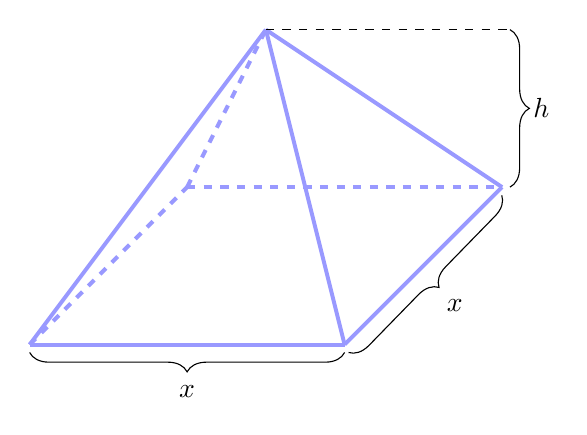
\begin{tikzpicture}
\draw[line width = 0.5mm,  color = blue!40] (0,0) -- (4,0);
\draw[line width = 0.5mm,  color = blue!40] (0,0) -- (3,4);
\draw[line width = 0.5mm,  color = blue!40] (4,0) -- (3,4);
\draw[line width = 0.5mm,  color = blue!40] (6,2) -- (3,4);


\draw[line width = 0.5mm,  color = blue!40] (4,0) -- (6,2);

\draw[line width = 0.5mm, dashed,  color = blue!40] (0,0) -- (2,2);
\draw[line width = 0.5mm, dashed,  color = blue!40] (2,2) -- (6,2);
\draw[line width = 0.5mm, dashed,  color = blue!40] (2,2) -- (3,4);
\draw[line width = 0.2mm, dashed] (3,4) -- (6.1,4);


\draw [decorate,decoration = {brace,mirror,amplitude = 7pt}] (0,-0.1) --  (4,-0.1);
\draw [decorate,decoration = {brace,mirror,amplitude = 7pt}] (4.05,-0.1) --  (6,1.9);
\draw [decorate,decoration = {brace,mirror,amplitude = 7pt}] (6.1,2) --  (6.1,4);

\node at (2,-0.6) {$x$};
\node at (5.4,0.5) {$x$};
\node at (6.5,3) {$h$};
\end{tikzpicture}
\caption{Pyramide med kvadratisk bund}
\label{fig:pyramide}
\end{figure}
\begin{enumerate}[label=\roman*)]
\item Rumfanget af en pyramide er givet ved $R = (b\cdot l\cdot h)/3$, hvor $l$ er længden af pyramiden, $b$ er bredden af pyramiden og $h$ er højden af pyramiden. Hvad er rumfanget af pyramiden på Fig. \ref{fig:pyramide}.
\item Vi skal bestemme overfladearealet af en af de fire overfladetrekanter. Brug Pythagoras' sætning samt Fig. \ref{fig:pyramide2} til at argumentere for, at overfladeareal af en af de fire sidetrekanter er givet ved 
\begin{align*}
O_T = \frac{x\cdot\sqrt{\frac{x^2}{4}+h^2}}{2},
\end{align*}
og konkludér, at det samlede overfladeareal af pyramiden må være givet ved 
\begin{align*}
O_P = 2\cdot x\cdot \sqrt{\frac{x^2}{4}+h^2}.
\end{align*}
\begin{figure}[H]
\centering
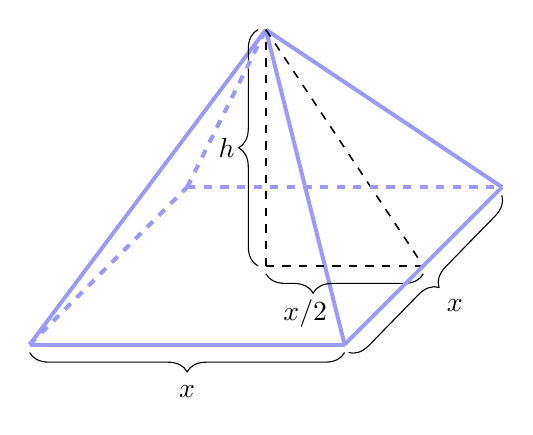
\begin{tikzpicture}
\draw[line width = 0.5mm,  color = blue!40] (0,0) -- (4,0);
\draw[line width = 0.5mm,  color = blue!40] (0,0) -- (3,4);
\draw[line width = 0.5mm,  color = blue!40] (4,0) -- (3,4);
\draw[line width = 0.5mm,  color = blue!40] (6,2) -- (3,4);

\draw[line width = 0.2mm, dashed] (3,1) -- (3,4);
\draw[line width = 0.2mm, dashed] (3,1) -- (5,1);
\draw[line width = 0.2mm, dashed] (3,4) -- (5,1);

\draw[decorate,decoration = {brace,amplitude = 7pt}] (3-0.1,1) -- (3-0.1,4);
\draw[decorate,decoration = {brace,mirror,amplitude = 7pt,aspect = 0.3}] (3,1-0.1) -- (5,1-0.1);

\draw[line width = 0.5mm,  color = blue!40] (4,0) -- (6,2);

\draw[line width = 0.5mm, dashed,  color = blue!40] (0,0) -- (2,2);
\draw[line width = 0.5mm, dashed,  color = blue!40] (2,2) -- (6,2);
\draw[line width = 0.5mm, dashed,  color = blue!40] (2,2) -- (3,4);



\draw [decorate,decoration = {brace,mirror,amplitude = 7pt}] (0,-0.1) --  (4,-0.1);
\draw [decorate,decoration = {brace,mirror,amplitude = 7pt}] (4.05,-0.1) --  (6,1.9);


\node at (2,-0.6) {$x$};
\node at (5.4,0.5) {$x$};
\node at (2.5,2.5) {$h$};
\node at (3.5,0.4) {$x/2$};
\end{tikzpicture}
\caption{Pyramide med kvadratisk bund}
\label{fig:pyramide2}
\end{figure}
\item Udnyt, at vi ved, at det samlede overfladeareal skal være $1$km$^2$, således at 
\begin{align*}
O_P = 1 = 2\cdot x\cdot \sqrt{\frac{x^2}{4}+h^2},
\end{align*}
og brug dette til at vise, at 
\begin{align*}
h=\sqrt{\frac{1}{4\cdot x^2}-\frac{x^2}{4}}.
\end{align*}
Det er vigtigt, at I viser alle mellemregninger.
\item Indsæt nu udtrykket for $h$ i udtrykket for rumfanget af pyramiden og plot rumfanget som funktion af $x$ på intervallet $[0,1]$. 
\item Bestem det $x$, der gør rumfanget af pyramiden maksimalt og bestem desuden den tilsvarende højde samt det maksimale rumfang.
\end{enumerate}
